\documentclass{article}

\usepackage{tikz}
\usetikzlibrary{positioning}
\usepackage{amsmath}

\begin{document}

% Message en ASCII

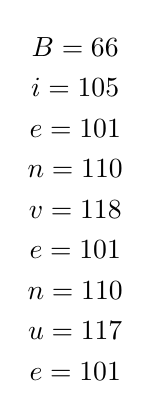
\begin{tikzpicture}
\node [minimum size = 0.5cm, inner sep = 0pt] (first) {$B = 66$};
\node [minimum size = 0.5cm, inner sep = 0pt, below = 0cm of first] (second) {$i = 105$};
\node [minimum size = 0.5cm, inner sep = 0pt, below = 0cm of second] (third) {$e = 101$};
\node [minimum size = 0.5cm, inner sep = 0pt, below = 0cm of third] (fourth) {$n = 110$};
\node [minimum size = 0.5cm, inner sep = 0pt, below = 0cm of fourth] (fifth) {$v = 118$};
\node [minimum size = 0.5cm, inner sep = 0pt, below = 0cm of fifth] (sixth) {$e = 101$};
\node [minimum size = 0.5cm, inner sep = 0pt, below = 0cm of sixth] (seventh) {$n = 110$};
\node [minimum size = 0.5cm, inner sep = 0pt, below = 0cm of seventh] (eighth) {$u = 117$};
\node [minimum size = 0.5cm, inner sep = 0pt, below = 0cm of eighth] (ninth) {$e = 101$};
\end{tikzpicture}

% Chiffrement

\vspace{1cm}

$f(x) = x^{e} \mod n$ avec $e = 7$ et $n = 8357$ \\

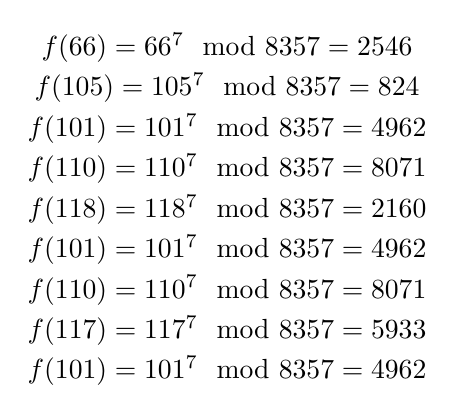
\begin{tikzpicture}
\node [minimum size = 0.5cm, inner sep = 0pt] (first) {$f(66) = 66^7 \mod 8357 = 2546$};
\node [minimum size = 0.5cm, inner sep = 0pt, below = 0cm of first] (second) {$f(105) = 105^7 \mod 8357 = 824$};
\node [minimum size = 0.5cm, inner sep = 0pt, below = 0cm of second] (third) {$f(101) = 101^7 \mod 8357 = 4962$};
\node [minimum size = 0.5cm, inner sep = 0pt, below = 0cm of third] (fourth) {$f(110) = 110^7 \mod 8357 = 8071$};
\node [minimum size = 0.5cm, inner sep = 0pt, below = 0cm of fourth] (fifth) {$f(118) = 118^7 \mod 8357 = 2160$};
\node [minimum size = 0.5cm, inner sep = 0pt, below = 0cm of fifth] (sixth) {$f(101) = 101^7 \mod 8357 = 4962$};
\node [minimum size = 0.5cm, inner sep = 0pt, below = 0cm of sixth] (seventh) {$f(110) = 110^7 \mod 8357 = 8071$};
\node [minimum size = 0.5cm, inner sep = 0pt, below = 0cm of seventh] (eighth) {$f(117) = 117^7 \mod 8357 = 5933$};
\node [minimum size = 0.5cm, inner sep = 0pt, below = 0cm of eighth] (ninth) {$f(101) = 101^7 \mod 8357 = 4962$};
\end{tikzpicture}

% Déchiffrement

\vspace{1cm}

$f'(x) = x^{d} \mod n$ avec $d = 4663$ et $n = 8357$ \\

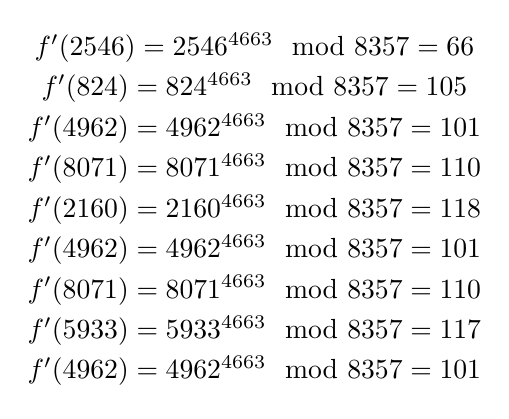
\begin{tikzpicture}
\node [minimum size = 0.5cm, inner sep = 0pt] (first) {$f'(2546) = 2546^{4663} \mod 8357 = 66$};
\node [minimum size = 0.5cm, inner sep = 0pt, below = 0cm of first] (second) {$f'(824) = 824^{4663} \mod 8357 = 105$};
\node [minimum size = 0.5cm, inner sep = 0pt, below = 0cm of second] (third) {$f'(4962) = 4962^{4663} \mod 8357 = 101$};
\node [minimum size = 0.5cm, inner sep = 0pt, below = 0cm of third] (fourth) {$f'(8071) = 8071^{4663} \mod 8357 = 110$};
\node [minimum size = 0.5cm, inner sep = 0pt, below = 0cm of fourth] (fifth) {$f'(2160) = 2160^{4663} \mod 8357 = 118$};
\node [minimum size = 0.5cm, inner sep = 0pt, below = 0cm of fifth] (sixth) {$f'(4962) = 4962^{4663} \mod 8357 = 101$};
\node [minimum size = 0.5cm, inner sep = 0pt, below = 0cm of sixth] (seventh) {$f'(8071) = 8071^{4663} \mod 8357 = 110$};
\node [minimum size = 0.5cm, inner sep = 0pt, below = 0cm of seventh] (eighth) {$f'(5933) = 5933^{4663} \mod 8357 = 117$};
\node [minimum size = 0.5cm, inner sep = 0pt, below = 0cm of eighth] (ninth) {$f'(4962) = 4962^{4663} \mod 8357 = 101$};
\end{tikzpicture}

\end{document}